\chapter{Quiz II (Version A)}
\label{ch:quiz}

\begin{preamble}
\begin{itemize}
\item You have 90 minutes to complete this examination.
\item Please answer all questions in the space provided with the
  question.  Clearly indicate your answers.
%% \item There are scratch pages at the end of the exam for your use. In no
%%   circumstance will anything you write on these pages count for or against
%%   your score on this exam.
\item You may refer to your one double-sided $8\frac{1}{2} \times 11$in
  sheet of paper with notes, but to no other person or source, during the
  examination.

\item You must open the exam in one and only one browser tab.  Not doing so could lead to loss of work.
%\item Your answers for this exam must be written in blue or black ink.

\end{itemize}
\end{preamble}

%\newpage
%\section{True or False}
%\input{true-false}

\newpage
\section{Recurrences}
Recall that $f(n)$ is $\Theta(g(n))$
if $f(n) \in O(g(n))$ and $g(n) \in O(f(n))$.
%Find tight bounds in
%terms of $\Theta$ for the following recurrences.


\begin{note}
You do not have to show your work, but it might help you get partial credit.
\end{note}

\begin{problem}[16.]
Give a closed-form
solution in terms of $\Theta$ for the following recurrences.  Also, state
whether the recurrence is dominated at the root, the leaves, or
equally at all levels of the recurrence tree.


\ask
Give closed form for  
$f(n) = 5f(n/5) + \Theta(n)$

%\hint[0.2] Here is a hint
%\explain[0.1] Some explanation.  Recall that Theta means big oh + omeca.

\sol
$\Theta (n \lg n)$.

\onechoice

\choice Balanced
\choice Leaves Dominated
\choice* Root dominated 



\ask
Give closed form for  
$f(n) = 3f(n/2) + \Theta(n^2)$

\sol
$\Theta(n^2)$

\onechoice  According to brick method, the recurrence is
\choice Balanced
\choice Leaves Dominated
\choice* Root dominated

\ask
$f(n) = f(n/2) + \Theta(\lg n)$

\sol
$\Theta (\lg^2 n)$

\onechoice  According to brick method, the recurrence is
\choice* Balanced
\choice Leaves Dominated
\choice Root dominated

\ask
$f(n) = 5f(n/8) +\Theta(n^{2/3})$

\sol
$\Theta(n^{\lg_8 5})$ (roughly $\Theta(n^{0.77})$) leaves.

\onechoice  According to brick method, the recurrence is
\choice Balanced
\choice* Leaves Dominated
\choice Root dominated

\end{problem}



\newpage
\section{Short Answers}

\begin{problem}[4.][Classes]

Lets say you are given a table that maps every student to the set of
classes they take.  

\ask

Fill in the algorithm below that returns all classes,
assuming there is at least one student in each class.  Your algorithm
must run in $O(m \log n)$ work and $O((\log m)(\log n))$ span, where
$n$ is the number of students and $m$ is the sum of the number of
classes taken across all students.    Note, our solution is one line.

\solfin

\begin{lstlisting}[numbers=none]
fun allClasses(T : classSet studentTable) : classSet = 
    ____ Table.reduce Set.union Set.empty T ____

\end{lstlisting}

\end{problem}

\begin{problem}[5.][Shortest Weighted]

Given a graph with integer edge weights between $1$ and $5$
(inclusive), you want to find the shortest \emph{weighted} path
between a pair of vertices. 

\ask
How would you reduce this problem to the
shortest \emph{unweighted} path problem, which can be solved using
BFS?

\sol
Replace each edge with weight $i$ with a simple path of $i$ edges
each with weight $1$. Then solve with BFS.

\end{problem}


\begin{problem}[5.][Visit and Finish]

Recall the implementation of DFS shown in class using the \sml{visit}
and \sml{finish} functions. Select the correct answer for each of the
following statements, assuming DFS starts at $A$:

\begin{center}
  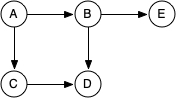
\includegraphics[scale=.7]{quiz/media/dfs-graph1.jpg}
\end{center}

\asktf
\texttt{visit D} could be called before \texttt{visit E}

\solt


\asktf
\texttt{visit E} could be called before \texttt{visit D}:
\solt

\asktf
\texttt{visit D} could be called before \texttt{visit C}
\solt

\asktf 
\texttt{finish A} could be called before \texttt{finish B}
\solf

\asktf
\texttt{finish D} could be called before \texttt{visit B}
\solt

\end{problem}

\begin{problem}[4.][Parallel Cycle Detection]
\ask
Describe in words how you would as part of star contraction 
efficiently detect that an undirected graph has a cycle.  \textbf{No more than two sentences.}

\sol
If during star contraction we find any self edges not involved in
contraction itself then there is a cycle.   However,
we need to be careful not to remove duplicate edges, and only to
contract along a single duplicate edge.

%% -4 if claim detecting duplicate edges is sufficient.  It is not sufficient because you can contract duplicate edges at the same time\\
%% %
%% -2 if say detect self edge, but do not point out issue with duplicates.\\
%% %
%% 0 for DFS, BFS, etc.
\end{problem}

\begin{problem}[6.][Star Contraction]
Select \textbf{every} type of graph listed below for which star
contraction will reduce the number of \textbf{edges} by a constant
factor in expectation in every round until fully reduced (and hence
imply $O(|E|)$ total work).  You can assume redundant edges between
vertices are removed.\\

\anychoice
\choice*  a graph in which all vertices have degree at most 2
\choice a graph in which all vertices have degree at most 3
\choice a graph in which all vertices have degree $\sqrt{|V|}$
\choice* a graph containing a single cycle (i.e. a forest with one additional edge)
\choice* the complete graph (i.e. an edge between every pair of vertices)
\choice any graph (still circle others if relevant)

\end{problem}


\newpage
\section{(Sets and Tables) Bingled}
%\section{(Sets and Tables) Bingled}

After forming your company Bingle to index the web allowing word
searches based on logical combination of terms (e.g. ``big'' and
``small''), you discover that there are already a couple companies out
there that do it....and lo-and-behold, they even have similar names.
You therefore decide to extend yours with additional features.  In
particular you want to support phrase queries: e.g. find all
documents where ``fun algorithms'' appears.

You decide the right way to represent the index is as a table of sets
where the keys of the table are strings (i.e. the words) and the
elements of the sets are pairs of values consisting of a document
identifier and an integer location in the document where the string
appears.  So, for example the following collection of three documents
with integer document identifiers:
%
\begin{quote}
\[
\begin{array}{ll}
\langle 
& (1, \cdm{``the~big~dog''}), 
\\
& (2, \cdm{``a~big~dog~ate~a~hat''}),
\\
& (3, \cdm{``i~read~a~big~book''})
\\
\rangle
\end{array}
\]
\end{quote}
~\\
the document index would be represented as
\[
\begin{array}{lll}
\cdm{idx} = & \{ & \cdm{``a''} \mapsto \cset{(2,0),(2,4),(3,2)}
\\
            &    &  \cdm{``big''} \mapsto \cset{(1,1),(2,1),(3,3)},
\\
            &   & \cdm{``dog''} \mapsto \cset{(1,2),(2,2)},
\\
            &   & \ldots
\\
            & \} &
\end{array}
\]

In particular you want to support the following interface
%
\begin{lstlisting}[language=Caml,numbers=none]
signature INDEX = sig
  type word = string
  type docId = int
  type index = docIdIntSet wordTable
  
  (* represents all documents and all locations where a phrase appears *)
  type docList

  val makeIndex : (docId * string) seq -> index    
  val find : index -> word -> docList
  val adj : docList * docList -> docList
  val toSeq : docList -> docId seq 
end
\end{lstlisting}
%
where, given an index \cd{idx},
%
\begin{lstlisting}[language=Caml,numbers=none]
toSeq (adj (find idx "210", find idx "rocks"))
\end{lstlisting}
%
would return a sequence of identifiers of documents
where ``210'' appears immediately before ``rocks'', and 
\\
\begin{lstlisting}[language=Caml,numbers=none]
toSeq (adj (find idx "Umut", adj (find idx "loves", find idx "climbing")))
\end{lstlisting}
~\\
would return a sequence of identifiers of documents
where the phrase ``Umut loves climbing'' appears.

\begin{problem}[8.]

\ask
Show the pseudocode for generating the index from the sequence of documents.
It should not be more than 8 lines of code and assuming all words have
length less than some constant, must run in $O(n \log n)$ work and
$O(\log^2 n)$ span, where $n$ is the total number of words across all
documents.    
%
You can use the function
%
\begin{lstlisting}[language=Caml,numbers=none]
toWords~:~string -> string seq
\end{lstlisting}
%
that breaks a text string into a sequence of words.

\solfin
\begin{lstlisting}[language=Caml, numbers=none]
type index = docIdIntSet wordTable

fun makeIndex (docs : (docId  * string) seq) : index =
  let
      ____ fun tagWords (id,doc) =                                     ____
      ____ let val words = toWords doc                                 ____
      ____ in                                                          ____
      ____ Seq.tabulate (fn i = (nth i words, (id, i)) (length words)  ____
      ____ end                                                         ____

      ____ val allPairs = Seq.flatten (Seq.map tagWords docs)          ____

      ____ val wordTable = Table.collect allPairs                      ____
      ____                                                             ____
      ____                                                             ____
      ____                                                             ____
      ____                                                             ____
in                  
    ____ Table.map Set.fromSeq wordTable                               ____
end
\end{lstlisting}
\end{problem}

\begin{problem}[8.]

Show code for a function \texttt{adj(docList1, docList2)} that given
two docLists returns a docList in which those two words
are adjacent.  For example for the index generated from the documents
above, 
\begin{lstlisting}[language=Caml,numbers=none]
toSeq(adj(find idx "a", find idx "big")) 
\end{lstlisting}
would return
$\cseq{2, 3}$.  For full credit \texttt{adj} must be an associative operator.

\ask
Define the \sml{docList} type and implement the function \sml{adj} as defined above.
You might find the function \sml{setmap} useful. The solution should
only be a few lines of code.
\begin{lstlisting}[numbers=none]
fun setmap f s = Set.fromSeq (Seq.map f (Set.toSeq s)) 
\end{lstlisting}


\solfin
\begin{lstlisting}[language=Caml,numbers=none]
type docList = (docIdIntSet) * int

fun adj (____      (d1,l1)      ____ , ____     (d2,l2)      ____ )  : docList = 
  let 
      ____ val d2' = setmap (fn (d,i) = (d, i-l1)) d2                     ____
  in  
      ____ (Set.intersection (d1,d2'), l1+l2)                             ____
  end
\end{lstlisting}


%% (* FYI: not part of exam *)
%% fun find idx word = 
%%   case Table.find idx word =>
%%     NONE => (Set.empty(), 1)
%%   | SOME d => (d, 1)
   
\end{problem}



\newpage
\section{(Shortest Paths) Dijkstra and A*}
%\section{(Shortest Paths) Dijkstra and A*}
%%\section{(Shortest Paths) Dijkstra and A*}
%%\section{(Shortest Paths) Dijkstra and A*}
%\input{../../../shortest-paths/dijkstra-astar}

\begin{problem}[6.]

Consider the graph shown below, where the edge weights appear next to
the edges and the heuristic distances to vertex $G$ are in parenthesis
next to the vertices.
\begin{center}
  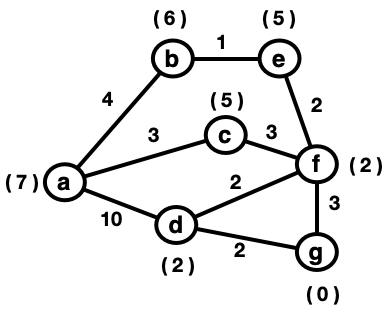
\includegraphics[scale=.75]{quiz/media/graph.jpg}
\end{center}

\ask
Show the order in which vertices are visited by Dijkstra when the source
vertex is $A$.
\sol
A C B E F D G


\ask Show an order in which vertices are visited by $A^*$ when
the source vertex is $A$ and the destination vertex is $G$.

\sol
A C F G 

\end{problem}

\begin{problem}[4.]

\ask
What is the key reason you would choose to use $A^*$ instead of
Dijkstra's algorithm?

\sol
You can use $A^*$ if you want the shortest path to only a single goal vertex,
and not all shortest paths. $A^*$ can be much more efficient, as it tries to
move toward the goal more directly, skipping many more vertices.
\end{problem}

\begin{problem}[5.]
\ask
Show a $3$-vertex example of a graph on which Dijkstra's algorithm always
fails. Please clearly identify which vertex is the source.

\sol
\begin{verbatim}
         A 
        / \
   x=4 /   \ y=-2   x+y < z < x guarantees failure
      /     \       x+y < z <= x may fail depending on the input order
    S ------- B
        z=3
\end{verbatim}
\end{problem}


\begin{problem}[6.]

Consider the graph shown below, where the edge weights appear next to
the edges and the heuristic distances to vertex $G$ are in parenthesis
next to the vertices.
\begin{center}
  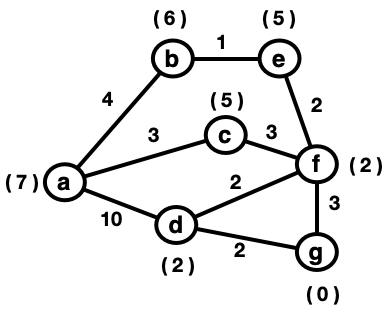
\includegraphics[scale=.75]{quiz/media/graph.jpg}
\end{center}

\ask
Show the order in which vertices are visited by Dijkstra when the source
vertex is $A$.
\sol
A C B E F D G


\ask Show an order in which vertices are visited by $A^*$ when
the source vertex is $A$ and the destination vertex is $G$.

\sol
A C F G 

\end{problem}

\begin{problem}[4.]

\ask
What is the key reason you would choose to use $A^*$ instead of
Dijkstra's algorithm?

\sol
You can use $A^*$ if you want the shortest path to only a single goal vertex,
and not all shortest paths. $A^*$ can be much more efficient, as it tries to
move toward the goal more directly, skipping many more vertices.
\end{problem}

\begin{problem}[5.]
\ask
Show a $3$-vertex example of a graph on which Dijkstra's algorithm always
fails. Please clearly identify which vertex is the source.

\sol
\begin{verbatim}
         A 
        / \
   x=4 /   \ y=-2   x+y < z < x guarantees failure
      /     \       x+y < z <= x may fail depending on the input order
    S ------- B
        z=3
\end{verbatim}
\end{problem}


\begin{problem}[6.]

Consider the graph shown below, where the edge weights appear next to
the edges and the heuristic distances to vertex $G$ are in parenthesis
next to the vertices.
\begin{center}
  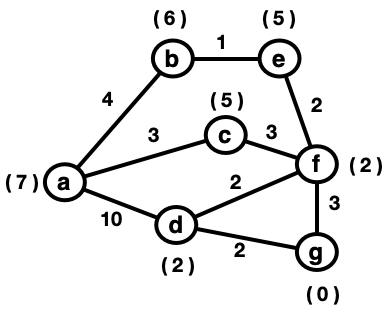
\includegraphics[scale=.75]{quiz/media/graph.jpg}
\end{center}

\ask
Show the order in which vertices are visited by Dijkstra when the source
vertex is $A$.
\sol
A C B E F D G


\ask Show an order in which vertices are visited by $A^*$ when
the source vertex is $A$ and the destination vertex is $G$.

\sol
A C F G 

\end{problem}

\begin{problem}[4.]

\ask
What is the key reason you would choose to use $A^*$ instead of
Dijkstra's algorithm?

\sol
You can use $A^*$ if you want the shortest path to only a single goal vertex,
and not all shortest paths. $A^*$ can be much more efficient, as it tries to
move toward the goal more directly, skipping many more vertices.
\end{problem}

\begin{problem}[5.]
\ask
Show a $3$-vertex example of a graph on which Dijkstra's algorithm always
fails. Please clearly identify which vertex is the source.

\sol
\begin{verbatim}
         A 
        / \
   x=4 /   \ y=-2   x+y < z < x guarantees failure
      /     \       x+y < z <= x may fail depending on the input order
    S ------- B
        z=3
\end{verbatim}
\end{problem}


\newpage
\section{(Graphs) Strongly Connected Components}
%\section{(Graphs) Strongly Connected Components}

In this question, you will write 2 functions on directed graphs.
We assume that key comparisons take $O(1)$ work  and  that graphs are represented as:
\begin{lstlisting}[language=Caml, numbers=none]
type graph = vertexSet vertexTable
\end{lstlisting}


\begin{problem}[10.]
Given a directed graph $G = (V,E)$, its transpose $G^T$ is
another directed graph on the same vertices, with every edge flipped.
More formally, $G^T = (V,E')$, where
$$E' = \{(b,a)~|~(a,b) \in E \}.$$

\ask
Here is a skeleton of an SML definition for \cd{transpose} that computes
the transpose of a graph. Fill in the blanks to complete the implementation.
Your implementation must have $O(|E| \log |V|)$ work and $O(\log^2 |V|)$
span.

\solfin

\begin{lstlisting}[language=Caml,numbers=none]
function transpose (G : graph) : graph = 
let
  val S = vertexTable.toSeq(G)    

  function flip(u,nbrs) = Seq.map ____     (fn v.(v,u))     ____ (vertexSet.toSeq nbrs)

  val ET = Seq.flatten(Seq.map flip S
  val T = vertexTable.____  collect              ____  ET
in
  vertexTable.map ____ vertexSet.fromSeq T               ____
end
\end{lstlisting} 
\end{problem}


\begin{problem}[10.]
A \emph{strongly connected component} of a directed graph $G = (V,E)$ is a subset $S$ of $V$ such
that every vertex $u \in S$ can reach every other vertex $v \in S$ (i.e.,
there is a directed path from $u$ to $v$), and such that no other vertex in
$V$ can be added to $S$ without violating this condition. Every vertex
belongs to exactly one strongly connected component{} in a graph.

\ask
Implement the function:
\begin{lstlisting}[language=Caml,numbers=none]
val scc~:~graph * vertex -> vertexSet
\end{lstlisting}
such that \cd{scc(G,v)} returns the strongly connected component{} containing $v$. You may assume
the existence of a function:
\begin{lstlisting}[language=Caml,numbers=none]
val reachable: graph * vertex -> vertexSet
\end{lstlisting}
such that \cd{reachable(G,v)} returns all the vertices reachable from $v$
in $G$. Not including the cost of \cd{reachable}, your algorithm must
have $O(|E|\log|V|)$ work and $O(\log^2 |V|)$ span.  You might find
\cd{transpose} useful and can assume the given time bounds.


\solfin
\begin{lstlisting}[language=Caml,numbers=none]
fun scc ($G$ : graph, v : vertex) : vertexSet = 
    ____  vertexSet.intersection(reachable(G,v),}                 ____
    ____ reachable(transpose(G,v)))}                              ____
\end{lstlisting}

\end{problem}



\newpage
\section{(MST) MST and Tree Contraction}
%\section{(MST) MST and Tree Contraction}

In \emph{SegmentLab}, you implemented Bor\r{u}vka's algorithm that
interleaved star contractions and finding minimum weight edges.  In
this question you will analyze Bor\r{u}vka's algorithm more carefully.

We'll assume throughout this problem that the edges are undirected,
and each edge is labeled with a unique identifier ($\ell$). The
weights of the edges do not need to be unique, and $m = |E|$ and $n =
|V|$.

\begin{lstlisting}[language=Caml, numbers=none]
(* returns the set of edges in the minimum  spanning tree of G *)

MST (G = (V,E)) = 
  if |E| = 0 then {}
  else let
    F = {min weight edge incident on v : v in V}
    (V',P) = contract each tree in the forest (V,F) to a single vertex
                  V' = remaining vertices
                  P = mapping from each v in V to its representative in V'
    E' = { (P_u, P_v, l) : (u, v,  l) in E  |  P_u <> P_v }
  in 
    MST (G' = (V',E')) union {l : (u,v,l) in F}
  end
\end{lstlisting}

\begin{problem}
\ask[4.]
Show an example graph with $4$ vertices in which \cd{F} will not include all
the edges of the MST.  Specify the graph as a set of vertices and edges, e.g., $V = \{0, 1, 2\}$ and $E = \{\{0,1\}, \{0,2\}\}$.

\sol
\begin{verbatim}
      3
   o --- o
 1 |     | 2
   o     o
\end{verbatim}

\ask[4.]
Prove that the set of edges $F$ must be a forest (i.e. $F$ has no cycle).

\sol
Answer 1: The MST does not have a cycle (it is a tree) and F is a subset of F
so it can't have a cycle.

Answer 2: AFSOC that there is a cycle.  Consider the maximum weight
edge on the cycle.  Neither of its endpoints will choose it since they
both have lighter edges.  Contradiction.
\end{problem}

\newpage

\begin{problem}[4.]
\ask
Suggest a technique to efficiently contract the forest in parallel.
What is a tight asymptotic bound for the work and span of your contract,
in terms of $n$? Explain briefly. Are these bounds worst case or
expected case?

\sol
Use star contraction as described in class. Since in contraction a tree
will always stay a tree, the number of edges must go down with the number
of vertices. Therefore total work will be $O(n)$ and span will be
$O(\log^2 n)$ in expectation.
\end{problem}

\begin{problem}[4.]
\ask
Argue that each recursive call to \sml{MST} removes, in the worst
case, at least \emph{half} of the vertices; that is, $|V'| \leq \frac{|V|}{2}$.

\sol
Every vertex will join at least one other vertex. Since edges have
two directions, at least $n/2$ of them must be selected, which will remove
at least $n/2$ vertices ($n = |V|$).
\end{problem}

\begin{problem}[4.]
\ask
What is the maximum number of edges that could remain after one step
(i.e. what is $|E'|$)? Explain briefly.

\sol
$m - n/2$ since at least $n/2$ edges are removed, as described in
previous answer.
\end{problem}

\begin{problem}[5.]
\ask
What is the expected work and span of the overall algorithm in terms of
$m$ and $n$? Explain briefly. You can assume that calculating $F$ takes
$O(m)$ work and $O(\log n)$ span.

\sol
Since vertices go down by at least a factor of $1/2$ on each round,
there will be at most $\log n$ rounds.  The cost of each round is
dominated by calculating $F$, $O(m)$ work and $O(\log n)$ span and the
contraction of forests $O(n)$ work and $O(\log^2 n)$ span.
Multiplying the max of each of these by $\log n$ gives $O(m \log n)$ work
and $O(\log^3 n)$ span.
\end{problem}


